\documentclass[a4paper,10pt]{article}
\usepackage[italian]{babel}
\usepackage[T1]{fontenc}
\usepackage[utf8]{inputenc}
\usepackage{amsmath}
\usepackage{amsthm}
\usepackage{amsfonts}
\usepackage{color}
\usepackage{bbm}
\usepackage{datetime}
\usepackage[colorlinks=true]{hyperref}
\usepackage{graphicx}
\usepackage{verbatim}
\usepackage{titlepic}
%\usepackage{physics}
\usepackage{subfigure}
\usepackage{float}

\newcommand{\abs}[1]{\lvert#1\rvert}

\begin{document}

 \title{\sc Homework 1}
\author{\sc Alice Schirinà}
\maketitle
	
\noindent Sono dati due file di testo, \textit{data1.txt} e \textit{data2.txt}, ciascuno dei quali organizzato in tre colonne di dati (per esempio $T$, $U_1$ e $U_2$) che rappresentano rispettivamente il tempo di misura e le misure delle osservabili $U_i$ ($i=1,2,3,4$). 
\section{Analisi a blocchi}
Supponiamo in un primo momento che i dati siano indipendenti e calcoliamone la media e l'errore:
\begin{equation*}
\langle U_i \rangle_{ind} = \frac{1}{N} \sum_{i}^{N} {U_i}
\end{equation*}
\begin{equation*}
\sigma_{i,ind}=\sqrt{\langle U_i^2 \rangle - \langle U_i \rangle ^2}
\end{equation*}
dove $N$ rappresenta il numero complessivo di dati per osservabile, in questo caso $N=100000$. In questo modo otteniamo i  seguenti risultati:
\medskip 
\begin{table}[H]
	\centering
	\begin{tabular}{rc} 
	\hline
	$\langle U_i  \rangle_{ind} $      &	$\sigma _{i,ind}$  \\
	\hline
	$2.135503$       & $0.001643$  \\
	$1.164563$       & $0.000434$  \\
	$-0.069248$      & $0.001884$  \\
	$2.031675$       & $0.002164$  \\
	\hline
	\end{tabular}
	%\caption{Medie ed errori per dati indipendenti}
\end{table}
\medskip
\noindent Vogliamo ora eseguire un'analisi a blocchi per tenere in considerazione la correlazione tra i dati. Generiamo, quindi, i blocchi di dati definendo la relazione per ricorrenza:
\begin{eqnarray*}
	U^{(1)}(t)&=&\frac{1}{2} [U_i(2t-1)+U_i(2t)]\\
	U_i^{(k)}(t)&=&\frac{1}{2}[U_i^{(k-1)}(2t-1)+U_i^{(k-1)}(2t)]
\end{eqnarray*}
\medskip
cosicché a ogni iterazione $k$ il numero dei dati si dimezza ($N/2$, $N/4$, etc). \\
Calcoliamo nuovamente la media usuale e l'errore sui dati come segue:
\begin{equation}
	\sigma_i(k)=\sqrt{\frac{\langle U_i^2 \rangle_k - \langle U_i \rangle_k ^2}{N-1}}
\end{equation}
in cui la media ed $N$ sono rispettivamente la media e il numero di dati nel blocco. 
Mostriamo in figura gli andamenti degli errori in funzione di $k$.
\medskip
%grafico sigma
\begin{figure}[H]
	\centering 
	\subfigure[{Andamento $\sigma_1$ in funzione di $k$}]%\label{fig:libraryvoid}
	{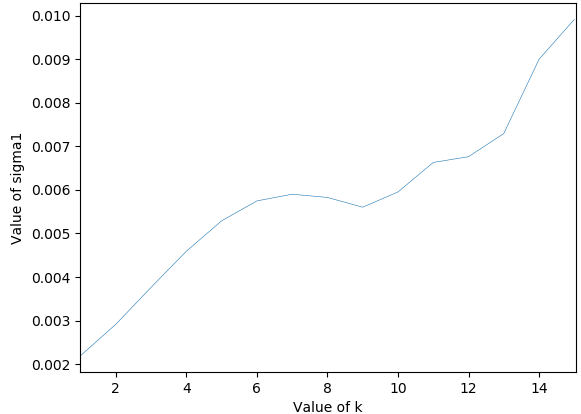
\includegraphics[width=0.44\linewidth]{graficoSigmaU1linea}}\qquad\qquad
	\subfigure[{Andamento $\sigma_2$ in funzione di $k$}]%\label{fig:board}
	{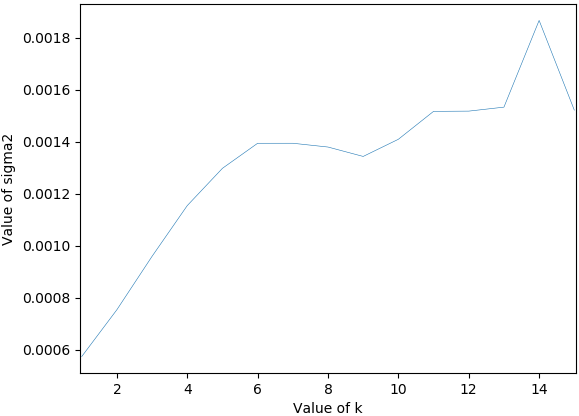
\includegraphics[width=0.44\linewidth]{graficoSigmaU2linea}}\qquad\qquad
	%\caption{Andamento degli errori in funzione di k}
	\subfigure[{Andamento $\sigma_3$ in funzione di $k$}]%\label{fig:libraryvoid}
	{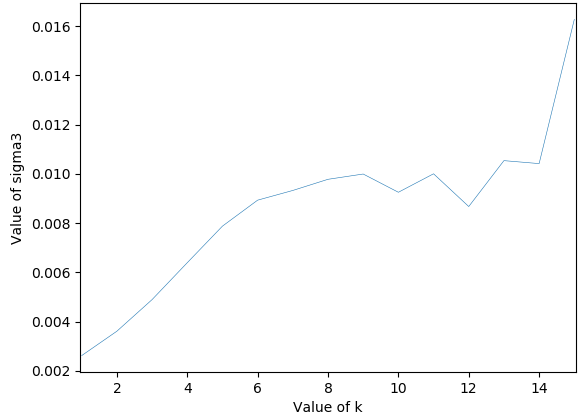
\includegraphics[width=0.44\linewidth]{graficoSigmaU3linea}}\qquad\qquad
	\subfigure[{Andamento $\sigma_4$ in funzione di $k$}]%\label{fig:board}
	{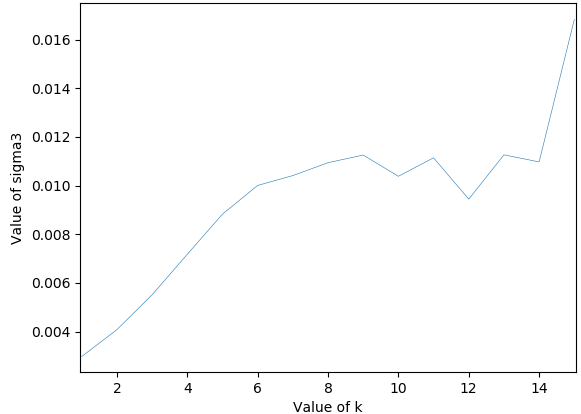
\includegraphics[width=0.44\linewidth]{graficoSigmaU4linea}}\qquad\qquad
	%\caption{Andamento degli errori in funzione di k}
\end{figure}
\medskip
\noindent Come possiamo osservare l'errore si stabilizza intorno a $k=6$. Scegliamo, quindi, questo valore di $k$ per ottenere una stima dell'errore per ognuna delle osservabili.
\medskip 
%tabella sigma 4 valori
\begin{table}[H]
	\centering
	\begin{tabular}{cl} 
	\hline
	Osservabile      &	Stima di $\sigma _{i}$  \\
	\hline
	$U_1$      & $0.005901$  \\
	$U_2$      & $0.001394$  \\
	$U_3$      & $0.009327$  \\
	$U_4$      & $0.010939$  \\
	\hline
%	\caption{Stima delle $\sigma_i$}
	\end{tabular}
\end{table}
\newpage
\section{Funzione di autocorrelazione}
Calcoliamo ora la funzione di autocorrelazione per ognuna delle variabili:
\begin{equation}
C(k)=\frac{1}{N-k} \sum_{j=1}^{N-k} (U(j+k)-\bar{U})(U(j)-\bar{U})
\end{equation}
Abbiamo simulato l'andamento della funzione fino a $k=500$. \\
%figure C(k)
\begin{figure}[H]
	\centering 
	\subfigure[{Andamento $C_1(k)$ in funzione di $k$}]%\label{fig:libraryvoid}
	{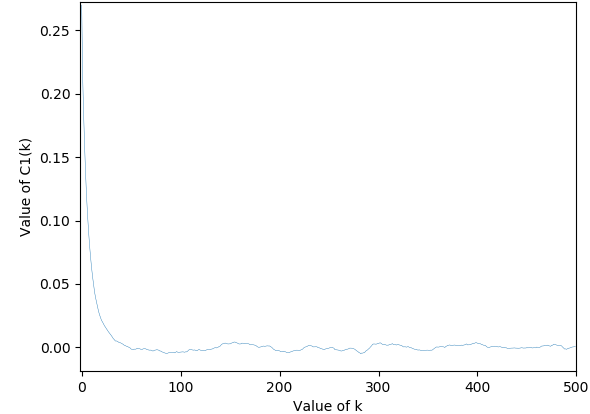
\includegraphics[width=0.44\linewidth]{CK1}}\qquad\qquad
	\subfigure[{Andamento $C_2(k)$ in funzione di $k$}]%\label{fig:board}
	{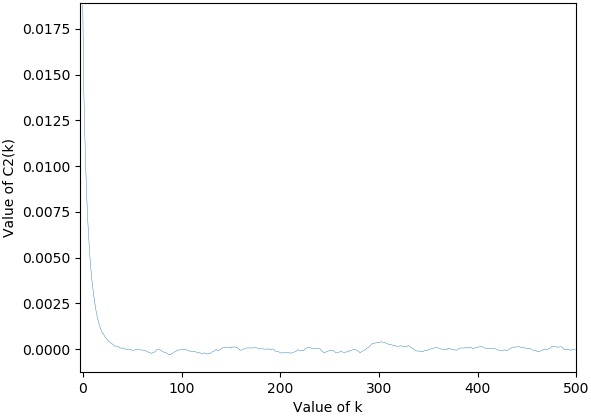
\includegraphics[width=0.44\linewidth]{CK2}}\qquad\qquad
	%\caption{Andamento degli errori in funzione di k}
	\subfigure[{Andamento $C_3(k)$ in funzione di $k$}]%\label{fig:libraryvoid}
	{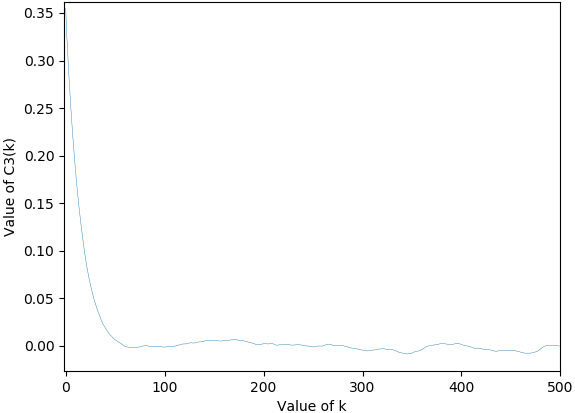
\includegraphics[width=0.44\linewidth]{CK3}}\qquad\qquad
	\subfigure[{Andamento $C_4(k)$ in funzione di $k$}]%\label{fig:board}
	{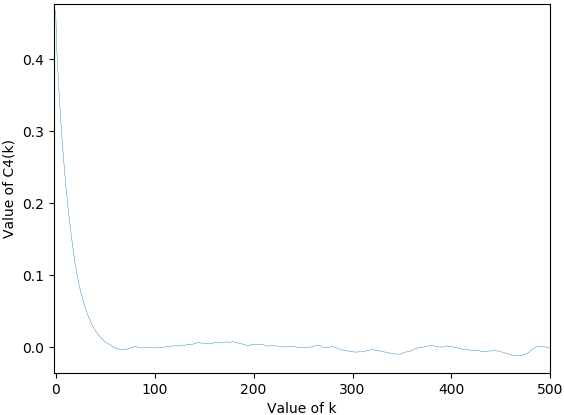
\includegraphics[width=0.44\linewidth]{CK4}}\qquad\qquad
	%\caption{Andamento degli errori in funzione di k}
\end{figure}
\medskip
\noindent Come possiamo osservare, a partire da un certo $k$ nell'intervallo tra $40$ e $60$, la curva tocca lo zero.\\  
Calcoliamo poi il corrispondente $\tau_{int}$ secondo:
\begin{equation}
\tau_{int}= \frac{1}{2} + \sum_{k=1}^{k_{max}} \frac{C(k)}{C(0)}
\end{equation}
dove per $k_{max}$ abbiamo considerato l'ultimo $k$ per cui la funzione $C(k)$ è ancora positiva.
\medskip
%tabella kmax tauint per ogni variabile
\begin{table}[H]
	\centering
	\begin{tabular}{ccc} 
	\hline
	Osservabile   & $k_{max}$  &  $\tau _{int}$  \\
	\hline
	$U_1$   	  &  $47$ &  $7.069802$  \\
	$U_2$         &  $43$ &  $5.712427$  \\
	$U_3$         &  $59$ &  $14.166401$  \\
	$U_4$         &  $58$ &  $13.406710$  \\
	\hline
	\end{tabular}
\end{table}
\medskip
Utilizziamo i tempi di autocorrelazione per stimare gli errori sul campione medio di $U_i$:
\begin{equation}
\sigma= \sqrt{\frac{C(0)}{N}2\tau_{int}}
\end{equation}
\medskip
e riportiamo in tabella il confronto tra gli errori appena ottenuti e quelli della sezione precedente per ogni variabile.
\medskip 
%tab sigmablock e sigmautoc
\begin{table}[H]
	\centering
	\begin{tabular}{cll} 
	\hline
	Osservabile & $\sigma(6)$      & $\sigma_{i}(\tau_{int})$  \\
	\hline
	$U_1$  &   $0.005901$   & $0.006177$  \\
	$U_2$  &   $0.001394$	& $0.001466$  \\
	$U_3$  &   $0.009327$	& $0.010029$   \\
	$U_4$  &   $0.010939$	& $0.011206$   \\
	\hline
	\end{tabular}
\end{table}
\medskip

\section{Metodo Jackknife}
Nell'analisi a blocchi ogni blocco contiene $N/2^k$ misure (con $k$ numero dell'iterazione) e l'errore si stabilizza intorno a $k=7$. Quindi, partendo dagli $N=100000$ dati iniziali, dovremmo raggruppare $2^k$ misure con dimensione massima per blocco pari a $512$ per avere blocchi di dimensione $N/2^k$. Riorganizziamo allora i dati in blocchi di $2000$ (circa quattro volte $512$), potendo assumere che essi siano scorrelati.\\
Su questi nuovi dati calcoliamo la variabile rapporto:
\begin{equation}
R_i=\frac{\langle U_i \rangle}{\langle U_1 \rangle}
\end{equation}
dove $i=2,3,4$. Quindi calcoliamo l'errore come segue:
\begin{equation}
\sigma_R = \left[ \frac{N-1}{N} \sum_{k=0}^{N-1} (\hat{R}_{i,k}-R_i) \right]^{\frac{1}{2}}
\end{equation}
dove $R_i$ è il rapporto delle medie aritmetiche delle medie Jackknife, in formule:
\begin{eqnarray*}
	\hat{R}_{ave}&=&\frac{1}{N} \sum_{k=1}^N \hat{U}_k\\
	R_i&=&\frac{\hat{R}_{ave,i}}{\hat{R}_{ave,1}}
\end{eqnarray*}
e, infine, le medie Jackknife sono:
\begin{equation}
\hat{U_i}= \frac{1}{N-1} \sum_{\substack{k=1 \\ k \neq i}}^{N} U_k
\end{equation}
Confrontiamo l'errore così ottenuto con quelli calcolati con l'\textit{independent-error formula} e la \textit{worst-error formula}:
\begin{equation}
\sigma_{IEF,R_i}= \sqrt{R_i^2 \left( \frac{\sigma_1^2}{\langle U_1 \rangle^2} + \frac{\sigma_i^2}{\langle U_i \rangle^2}  \right)}
\end{equation}
\begin{equation}
\sigma_{WEF,R_i}= \sqrt{R_i^2 \left( \frac{\sigma_1}{\abs{\langle U_1 \rangle}} + \frac{\sigma_i}{\abs{\langle U_i \rangle}}  \right)^2}
\end{equation}
Da queste formule otteniamo i seguenti valori per gli errori sulle $R$:
\medskip
%errJK, IEF, WEF
\begin{table}[H]
	\centering
	\begin{tabular}{rlll} 
	\hline
	$R_i$ & $\sigma_{JK}$      & $\sigma_{IEF}$   & $\sigma_{WEF}$ \\
	\hline
	$0.545334$  &  $0.001012$	& $0.001720$  &  $0.002264$\\
	$-0.032428$  &  $0.004321$	& $0.004698$  &  $0.004790$\\
	$0.951379$  &  $0.006699$	& $0.005925$  &  $0.007999$\\
	\hline
	\end{tabular}
\end{table}
\medskip
\noindent Come ci aspettavamo gli errori ottenuti con la \textit{worst-error formula} sono una sovrastima dell'errore ottenuto con il metodo Jackknife. Anche l'errore con l'\textit{independent-error formula} in questo caso risulta essere una sovrastima.




\end{document}
